\section{Technical Details of the Optimizer}
\label{sec:tech-details}
The sections above describe my innovations in model construction and simulation, as well as the experimental data brought to bear on optimization. These data are used to parameterize NeuronUnit tests, one per measurement type.
For example the input resistance data for one neuron type in NeuroElectro, or one specific neuron in the Cell Types database, is passed to an \textit{InputResistanceTest} defined in NeuronUnit.
This test "asks" the model to generate a corresponding simulation, measures the input resistance in this simulation output, and then assesses model/data agreement, resulting in a score.
These mechanics have been described at length previously in \cite{omar2014collaborative}, \cite{gerkin_neuronunit}, and \cite{birgiolas2019towards}.

\begin{figure}
\begin{center}
	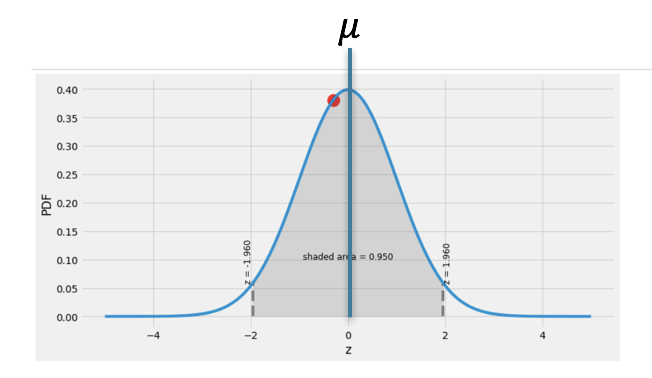
\includegraphics{figures/normal_distribution}
    \caption[Z-scores for NeuronUnit Tests]{As discussed in the section \ref{sec:neuronunit}, error functions were evaluated with the assistance of the \emph{NeuronUnit} library.
    This involves obtaining an experimental distribution over electrophysiology feature measurements for a cell type, measuring corresponding model output features and then locating those features in that experimental distribution. 
    Scores that are closer to the experimental mean are identified as low error.
	The Z-score encodes this information; a Z-score of 0 is the lowest possible error.}
\end{center}
	
\end{figure}
%XXXX Something about Z-score vs RatioScore.

When doing sub threshold fitting with NeuroElectro data, its possible to use Z-scores, as discussed in pitfalls Z-scores enable one to assess biological plausibility of a fitted model, assuming that underlying data is normally distributed.  When the data is one single experiment RatioScore is used instead, this is the case for tests constructed from Allen Cell Types and BlueBrain Project data sources.

\begin{itemize}
    \item known Gaussian distribution $(\mu, \sqrt{\sigma}) = (100pA, 40pA)$
    \item normalized to 1: Z-score: 
        \subitem For example: An evaluated model returns $110pA$ as a rheobase current
        \subitem The value $110pA$ is mapped onto normalized distribution: $\frac{abs(110pA-\mu)}{\sqrt{\sigma^{2}}} = 0.25$
    \item $\log_{10}(1-0.25) $ 
    \item best fitness is $0.0$, worst fitness is arbitrary, for simplicity lets call it $100$.
        \subitem  $ error = $ abs(log-norm-score))$ = 0.12$ 
        \subitem $ fitnesses = collection(errors) $
\end{itemize}
%XXXX Enumerated list showing how data determines a Z-score (or a RatioScore) which then determines a norm-score, a log-norm-score, and the objective function result.

Here I will describe how I generate these scores concurrently for many parameterizations of the same model, and how the scores themselves guide subsequent parameterizations, i.e. how optima are reached.

% TODO
%XXXX Russell I need you to write a few paragraphs here about the mechanics of your optimizer.  Data Transport containers, evaluation, selection, etc.  You can skip over (or refer to) anything already written in the introduction, i.e. you can assume that mutation/crossover and such things are already understood.
I created two different DEAP optimization code bases, and slowly merged the two code bases together. Before creating NeuronUnit compatibility inside a branch of BluePyOpt, I crafted a DEAP NeuronUnit specific Optimizer. I will describe a few files that are mutual to both code-bases, and which are essential to the current state of play. A file $optimization_management.py$ contains logic and methods for managing complex optimization jobs. It contains logic for making the optimizer handle fixed both and modifiable model parameters, it also contains methods for random sampling of models, plotting models firing at multiples of rheobase, and logic for solving for finding the current required to cause a given number of spikes. I have also contributed many methods for converting between models and chromosomes, and chromosome to models.

%The method $instance_opt$ was able to instance $NUFeature_standard_suite$, and then by instantiating objective objects, it could aggregate Neuronunit scores, and 

A class NUFeature-standard-suite converts NeuronUnit Features to BluePyOpt objective functions. These classes contain a complicated nesting of fault handling statements, as there are many reasons why an sampled model return discontinuous membrane potentials, so values like NaN and infinity needed to be recast as poor optimizer scores. There are two flavors of $NUFeature_standard_suite$, one for supra-threshold experiments and another for at threshold or sub-threshold virtual experiments. These different virtual experiments utilize different feature extractors, and so it is natural to separate the source code into dedicated modules. Another reason for the test suite split is because each of these two types of virtual experiment has its own pattern of fault causing behavior (there are more ways for a model not to elicit multiple comparable spikes, there are less ways to produce un-comparable single spikes).
 
I also contributed a model-parameters.py file, which was a collection of Ordered dictionaries, that informed the optimizer what parameters are modifiable and what are their boundaries. Later, I would make this file and its methods inter-operable with BluePyOpts model parameters scheme.

%-- System of fault handling
%-- Recasting NeuronUnit scores into objective function values (e.g. log norm score)Aggregation of neuronunit scores into multi-objectives
%-- etc

Typical parameters for robust optimization were number of generations=$NGEN=150$, population size=$\mu=35$.
In other words, it took about $150$ generations to achieve convergence, and in each generation about $25$ individual parameter sets needed to be retained in order to achieve an acceptable balance between exploration of the parameter space and exploitation of favorable regions.
In some cases, values as small as $NGEN=10$ and $\mu=10$ were tolerable, for example when optimizing only low-dimensional cross-sections of parameter space.
In other cases, such as when the number of optimization objectives (i.e. the number of electrophysiological features being tested) was $NOBJ>25$, values as high as $NGEN=300$ and $\mu=100$ were required to obtain adequate results.

One potential goal is to maintain a diverse set of solutions (i.e. very different parameter sets that nonetheless each produce simulations that adequately match observed experimental measurements).
The optimization literature has developed many competing approaches for doing this \cite{deb2000fast}, but it usually involves  

Two popular algorithms, named IBEA and NSGA2, were investigated here.
% XXXX Russell write about why IBEA is better.
NSGA2 uses some additional ranking mechanisms, to re-weight the perceived value genetic fitnesses when chromosomes are chosen to breed according to "meta" constraints. One type of meta-constraint: "crowding distance", is a way of penalizing chromosomes that aggregate in clusters, as persistent cluster formation means that the GA becomes preoccupied with more limited regions of the solution space harming solution diversity. Another meta constraint "non-dominated sorting" re-weights chromosomes and improves likelihood of mating only if all of their fitness values go down together. Consistent with personal communication with \cite{van2007neurofitter} in neuronal model optimization adding in crowding distance and non-dominated sorting harms optimizer performance, the reason for this is unclear, but the result is persistent. It could be that the mechanism of domination, where initially only one fitness value goes down dramatically at the expense of others going up or staying the same, better facilitates uphill exploration. IBEA may better facilitate moving up over a hump or a "lip" to then, fall into gravity of error wells, were soon after all errors are able to fall together. The simpler select best algorithm (labelled IBEA) allows for single error domination effect to occur, as it IBEA performs no additional list sorting, and does not apply meta-constraints.

%Both resulted in similar solution quality, but this varied in a problem specific manner.

%I found that IBEA usually produced better results faster, although in some cases it yielded solutions that were overly dominated by performance on a single test, and thus it was difficult to trust this algorithm across the board.
%NSGA2 was thus used for the remainder of the results shown here.

\subsection{Similarities and Differences from Previous Approaches to Optimization}
Other labs have previously developed schemes to optimize neuron models, e.g. \cite{druckmann2007novel}.
I retained the conceptual insights of these approaches where they were useful for the problems at hand.
For example, I utilized a time-dependent mutation magnitude ($\eta$).
The idea is that big mutations are more helpful in the early stage of optimization, when it is important to explore the vast hyper-volume of parameter sets and get a general picture of the error surface, and that these mutations should be smaller during the later "refinement" stage of optimization, as the best solutions are approached.

Nearly all neuron optimization work (including this one) relies on the responses to somatically-injected current as the domain for optimization.

This is largely motivated by the existence of a common and simple experimental analogue using patch clamp (which drives experimental design for both the Allen Cell Types database and The Blue Brain Project portal).
But there are three different strategies for choosing the subset of these experiments that are recapitulated in optimization.
The first strategy involves blindly choosing a fixed set of current amplitudes (e.g. ascending 100 pA steps) from the data and probing the model with these, then comparing model and data within this subset.

The second strategy involves first identifying the rheobase current, and choosing multiples of or steps around that current for subsequent evaluation. This strategy was used not just in optimization, but also in the analysis and re-organization of existing ephys data.

The third strategy took place in when fitting to multiple model/experiment spike fits. The second strategy involved counting the number of spikes in experimental data, and directly searching the model for the minimum current required to cause the same spike number. With matching spike counts, both model and data were more readily comparable.
%with multi spiking waveforms could be compared by causing models to illicit the same number of spikes. 

The first strategy is more direct and slightly more rapid, but it is inefficient in terms of constraining the model, because all of the "action" in the F-I curve occurs above rheobase, but not too far above rheobase (i.e. not at currents that induce depolarization block).
Action potential waveforms are also more regular and consistent in shape when evaluated very near rheobase. 
% orphaned sentences:
%The second and third strategy thus use the data (and simulations) that are most informative in terms of constraining model parameters. 
%I use the third strategy though the plots of multiple spike fits seen later in the document.
%I use this second strategy throughout.

If one were to follow the second strategy, one must then decide how many current amplitudes (above rheobase) must be evaluated in order to adequately constrain model parameters.
For example, if the rheobase uniquely determined the entire F-I curve, and if all neurons showed an identical regular, non-accommodating spiking pattern, it would probably be sufficient to identify the rheobase current and move on. To the extent that this (poor) assumption is violated, various additional suprathreshold current injections will be needed. 

The third strategy approaches the problem differently, for every chromosome models are made to fire the same number of spikes as experiments. Disagreement in spike shape, and spike irregularity are only modulated by differences in model parameters. The consequences of these decisions are explored in the Results section.

\subsection{Feature Extraction}
Each NeuronUnit test used in the optimizer represents the evaluation of a single feature of simulated output, for example the Input Resistance.
I greatly extended the number of such features/tests covered by NeuronUnit in order to produce a rich, multi-objective optimizer that could capture important spiking dynamics and to obtain insights into what would be the most compact subset for subsequent use in unique identification of models.

\subsubsection{Elephant Features Test Suite}
Elephant \cite{elephant18} provides feature extraction capabilities for membrane potential time series expressed using the Neo library in Python \cite{davison_neo}.
Eight NeuronUnit tests (five used here) are derived from Elephant feature extraction, particularly those associated with passive membrane properties assessed with subthreshold stimuli, or action potential waveform properties assessed at rheobase.
Fundamental quantities such as capacitance or input resistance are among these are of  particular interest since they are not "emergent properties" of the model but are roughly predictable from the parameters of the model equations.

\subsubsection{Electrophysiology Feature Extraction Library (EFEL)}
%Most suprathreshold dynamics were summarized by descriptive statistics of patterns of action potentials. For example, the coefficient of variation of the inter-spike intervals in a spike train can serve as a measure of "burstiness". -- No EFEL has many spike shape qualities. as the noted well as spike train statistics. I'd say the ratio of spike train statistics to spike shape measurements is about 1:1.
The Blue Brain Project developed the Electrophysiology Feature Extraction Library (EFEL) to compute many such statistics from spike trains, and I used these to generate tests of suprathreshold dynamics for optimization.

\subsubsection{Allen Institute Software Development Kit (Allen SDK)}
The Allen Institute offers yet another set of tools for feature extraction, applying to both sub- and suprathreshold features of neuron responses to current injection.
The reason to use these in addition to the above is that some of these features are predicated on particular current stimuli (e.g. a stimulus that is exactly 20 pA stronger than the rheobase current).
Such stimuli either were or were not delivered to the various experimentally recorded neurons, and for the purposes of this thesis there is no going back and delivering additional ones.
Consequently, it makes sense to use features--and the stimuli that generate them--that can be directly compared to the recorded neurons.
For the biological neurons in the Allen Cell Types database, these features are available in the Allen SDK.
